% Super-Weights in Genomic Language Models — v6
% Tightened title and abstract; softened overstated claims; reconciled
% Evo1 numbers; rewritten Figure 3 caption; expanded limitations.
% Compatible with pdfLaTeX, XeLaTeX, and LuaLaTeX.
\documentclass[11pt]{article}

%% ---- engine-agnostic font setup ----
\usepackage[T1]{fontenc}
\usepackage{lmodern}
\usepackage[utf8]{inputenc}

%% ---- page geometry ----
\usepackage[margin=1in]{geometry}

%% ---- math ----
\usepackage{amsmath,amssymb}

%% ---- graphics ----
\usepackage{graphicx}
\graphicspath{{media/}}

%% ---- tables ----
\usepackage{booktabs,array,longtable}
\usepackage{caption}
\usepackage{float}

%% ---- hyperlinks ----
\usepackage{hyperref}
\hypersetup{colorlinks=true,linkcolor=blue,urlcolor=blue,citecolor=blue}

%% ---- misc ----
\usepackage{xcolor}
\usepackage{enumitem}
\usepackage[normalem]{ulem}

%% ---- paragraph spacing ----
\setlength{\parindent}{0pt}
\setlength{\parskip}{6pt}
\setlength{\emergencystretch}{3em}
\hbadness=10000
\sloppy

\begin{document}

\begin{center}
{\large\bfseries A Structural Predictor of Super-Weights Across
Genomic Language Model Architectures}

\vspace{6pt}
{\normalsize
Alexandros Tzanakakis\textsuperscript{1},
Aris Karatzikos\textsuperscript{1,2},
Ilias Georgakopoulos-Soares\textsuperscript{1,*}
}

\vspace{6pt}
{\small
\textsuperscript{1}Division of Pharmacology and Toxicology, College of
Pharmacy, The University of Texas at Austin, Dell Paediatric Research
Institute, Austin, TX, USA.\\
\textsuperscript{2}Department of Computer Science, College of Natural
Sciences, The University of Texas at Austin, Austin, TX, USA.\\
\textsuperscript{*}Corresponding author:
\href{mailto:ilias@austin.utexas.edu}{ilias@austin.utexas.edu}
}
\end{center}

\vspace{6pt}

\textbf{Abstract}

Super-weights---individual parameters whose ablation catastrophically
degrades large language model performance---have been characterised
in natural-language transformers, but whether they exist in genomic
language models, and how they relate to architecture, has not been
systematically studied. We scanned eight of the best genomic
language models spanning transformer decoders, encoder transformers,
state-space models, and hybrid architectures. We make three
contributions. First, we identify a closed-form, weight-only
structural predictor of candidate super-weight rows---the Frobenius
bound $\|U_k\|_F$ on the rank-1 gated-FFN amplifier---and show it
ranks the empirical super-rows at the top of their layer in three
independent gated-FFN transformer models (GENERator SwiGLU decoder,
DNABERT-2 GLU encoder, NTv3 encoder), from cold weights and zero
forward passes. The same predictor concentrates equally on candidate
rows in a StripedHyena hybrid (Evo1), but ablating those rows yields
$\Delta\mathrm{PPL} \approx 0$. The mechanism therefore separates
into a structural component (the gated-FFN amplifier; weight-only
predictable) and a systemic component (whether the surrounding mixer
preserves the candidate along its own residual coordinate). Second,
within the SW-positive models, super-weights encode nucleotide
composition rather than annotated regulatory grammar, with a
sign-reversed correlation between SW activation and ablation cost
between the eukaryotic ($r = {+}0.437$) and prokaryotic
($r = {-}0.710$) GENERator models; a sparse autoencoder trained on
prokaryotic residual-stream activations independently recovers the
same compositional axis. Third, ablating the SW ensemble in DNABERT-2
collapses splice-site recognition by $-25.5\%$ accuracy while leaving
histone-mark prediction intact, and the splice effect replicates in
NTv3 across five seeds ($\Delta\mathrm{MCC} = -0.119 \pm 0.054$,
$p = 0.008$). The SW neighbourhood is extremelly tolerant to pruning
and INT4 quantization compared with random rows, suggesting refined
SW-aware compression schemes are possible.

\textbf{Introduction}

Genomic language models use large-scale self-supervised learning to
decode the complex, overlapping vocabularies of DNA sequence and
predict regulatory, functional, and disease-relevant genomic
effects.\textsuperscript{1--3} They span diverse architectural
families, including autoregressive transformer decoders such as
GENERator\textsuperscript{4} and NTv3,\textsuperscript{5}
bidirectional encoder models such as DNABERT-2,\textsuperscript{6}
state-space and convolutional hybrids such as Evo1/Evo2,
\textsuperscript{7} Hyena-attention hybrids such as
HybridNA,\textsuperscript{8} and EMA-based architectures such as
MegaDNA.\textsuperscript{9} Their internal mechanisms remain largely
unresolved.

Recent work in natural language has identified rare super-weight
neurons whose ablation causes catastrophic model failure despite
comprising an infinitesimal fraction of total
parameters,\textsuperscript{10} and follow-up mechanistic
work\textsuperscript{11} has traced these to a directional quadratic
amplifier in early feed-forward layers. Whether analogous phenomena
exist in genomic language models, whether they generalise across
architectures, and whether they encode biological signal or purely
statistical sequence features has not been established.

Here we investigate super-weights across eight genomic language
models. Our central result is a closed-form, weight-only predictor
of candidate super-weight rows that holds across three independent
gated-FFN transformer architectures: the Frobenius bound
$\|U_k\|_F$ derived from the rank-1 outer-product structure of any
gated FFN identifies the empirical super-row at or near the top of
its layer in GENERator (SwiGLU decoder), DNABERT-2 (BertGatedLinearUnit
encoder), and NTv3 (Mistral-style encoder), without using any
training or inference data. The same predictor applied to Evo1
(StripedHyena hybrid) also concentrates on candidate rows, but
ablating those rows produces no measurable functional effect. We
interpret this dissociation as evidence that super-weight emergence
has two separable components: a structural property of the gated
FFN block (predictable from weights alone) and a systemic property
of the surrounding mixing operator (whether candidate concentrated
channels are preserved along their own residual coordinate
downstream). Within the SW-positive models we additionally
characterise what the super-weight encodes (nucleotide composition,
not biological regulatory grammar), document a sign-reversed
SW-activation/ablation-cost correlation between the eukaryotic and
prokaryotic GENERator models, and show that the immediate
neighbourhood of the SW row is unusually tolerant to pruning and
INT4 quantization---a property we term shadow redundancy.

\textbf{Results}

\medskip
\noindent\textbf{Super-weight existence across architectures}

We applied a unified detect-then-ablate protocol to eight models: a
single forward pass to identify the row in \texttt{down\_proj} (or
its architectural analogue) whose zeroing caused the largest
activation drop, followed by functional evaluation via held-out
perplexity and, for fine-tunable encoders, downstream task accuracy
(\textbf{Figure~\ref{fig:arch}}). All eight models passed the
detection stage with an identifiable candidate row above the layer
median; the models differ in whether the candidate is load-bearing.

In GENERator eukaryote 3B, the sweep converged on a single dominant
super-row at layer~4, row~2{,}371 (out\_max $= 375{,}361$;
in\_max $= 67{,}551$). This row contains 8{,}448 parameters
(approximately 0.0003\% of the model's $\sim 3$~billion weights);
ablating it increased perplexity from 3.40 to 785.5 ($+23{,}026\%$).
Ten randomly selected rows of identical size produced no measurable
effect ($\Delta$PPL $< 0.01\%$). A secondary super-row at the same
layer (row~1{,}522; out\_max $= 143{,}880$) produced an additional
but smaller effect when ablated sequentially. GENERator prokaryote
3B showed a comparable phenotype at layer~2, row~1{,}927
(out\_max $= 506{,}014$): ablation raised perplexity from 2{,}324 to
606{,}073 ($+25{,}975\%$), with random-row controls within 0.03\%
of baseline.

DNABERT-2 showed a qualitatively different pattern. The sweep
identified ten candidate super-rows concentrated around row~603 at
multiple encoder layers (layers 3, 5, 6, 7, 9; out\_max 137--945).
Zeroing these rows produced only a $+1.5\%$ perplexity increase
under masked-LM evaluation; the same ablation, applied to a
fine-tuned model, caused a $-25.5\%$ accuracy collapse on splice-site
recognition (see Functional Consequences). A Monte-Carlo proximity
analysis ($n = 50{,}000$ random sets; z-score $-1.19$, 12th
percentile) and a structured-random control matching the empirical
layer distribution and row-repetition pattern ($\Delta$acc
$-0.02\%$) confirmed that row identity, not layout, carries the
signal. NTv3, a second encoder model with a gated FFN, also showed a
distributed-ensemble dependency revealed by downstream evaluation:
across five splice-site fine-tuning seeds, SW-row ablation produced
$\Delta\mathrm{MCC} = -0.119 \pm 0.054$ ($t = -4.86$, $p = 0.008$
one-sample vs.\ zero, 5/5 seeds in the negative direction), with
random-row controls at the $3 \times 10^{-4}$ noise floor.

The SSM and hybrid models returned null functional results under the
same protocol. We focused detailed analysis on Evo1, the
StripedHyena member that loads in our standard environment (Evo2
requires a custom Singularity container; MegaDNA weights are gated).
Importantly, Evo1 is not a detection-stage negative: the activation
sweep finds a hotspot at layer~11, column~9{,}885 with multiple rows
at out\_max $\approx 10^6$, larger than DNABERT-2's peak. The
detection stage fires identically to the positive cases. However,
ablating the top-scoring row produces $\Delta$PPL $= 0.0\%$
(3.1127 $\rightarrow$ 3.1131; random-row controls $\approx 0$); the
candidate row is non-load-bearing despite the spike. HybridNA and
MegaDNA were tested by ablation only and produced $\Delta$PPL
$= -1.3\%$ and $+0.3\%$, indistinguishable from random. Caduceus
was not tested under ablation due to a CUDA-extension incompatibility;
static weight analysis showed a max/median ratio of $2.4\times$ with
no outliers, but Caduceus is not part of the protocol-symmetric
comparison. Within the four models we did evaluate under ablation,
the phenotype tracks architecture class: transformer decoders show
concentrated single-row dependencies, transformer encoders show
distributed ensembles revealed by downstream task ablation, and
StripedHyena shows detection-stage candidates that are not
load-bearing downstream.

\begin{figure}[H]
\centering
\includegraphics[width=\textwidth,height=0.62\textheight,keepaspectratio]{media/image_fig1.png}
\caption{\textbf{Detect-then-ablate protocol applied to eight genomic
language models.}
\textbf{(A)}~Peak activation magnitude (out\_max) of the dominant
weight row plotted against its normalised layer position. 
Filled markers indicate models with a positive ablation effect and open markers indicate models with a
detection-stage hotspot but null ablation effect.
\textbf{(B)}~Perplexity change ($\Delta$PPL\%) on ablation of the
candidate SW row (bars) versus an equal-norm random row (dots);
\textbf{(C--D)}~Location of the super-weight within the GENERator EUK
(C) and PROK (D) transformer stacks.}
\label{fig:arch}
\end{figure}

\medskip
\noindent\textbf{A weight-only structural predictor identifies
candidate super-rows in three gated-FFN transformer architectures}

For each output coordinate $k$ of a gated MLP, the contribution of
every hidden unit $i$ to coordinate $k$ admits a rank-1
outer-product bound that yields the Frobenius expression
\[
\|U_k\|_F
= \sqrt{\sum_{i=1}^{d_{\text{ffn}}}
  W_{\text{down}}[k,i]^2
  \cdot \|W_{\text{gate}}[i,:]\|^2
  \cdot \|W_{\text{up}}[i,:]\|^2},
\]
where $W_{\text{gate}}$, $W_{\text{up}}$, $W_{\text{down}}$ are the
three projection matrices of a gated FFN. The expression depends
only on weights, requires no forward pass or training data, and
ranks output coordinates by their structural amplification capacity.
We applied this predictor to four gated-FFN architectures and
compared the result to the empirically identified SW rows.

\textit{GENERator EUK and PROK.}
SW rows ranked first among all 3{,}072 output coordinates at the
step-up layer in both models. EUK row~2371 reached
$\|U_k\|_F = 215.86$ versus a layer median of 17.63 ($12\times$
above median; rank 1/3{,}072), and EUK row~1522 ranked second
($4.6\times$). PROK row~1927 reached $\|U_k\|_F = 2{,}648$ versus a
median of 148 ($18\times$; rank 1/3{,}072). The SW rows were
identified independently by activation magnitude during inference;
their simultaneous top ranking in the weight-space audit indicates
that both measures reflect the same high-gain amplifier structure.

\textit{DNABERT-2.}
The formula applies directly to DNABERT-2's
\texttt{BertGatedLinearUnitMLP}, whose \texttt{gated\_layers} packs
gate and up projections on adjacent row blocks of a single matrix.
Applied cold-weights, the predictor places 9 of the 10 known SW
rows in the top 3 of their layer (median rank 1.4 in
$d_{\text{model}} = 768$). The single outlier is layer~7 row~603 at
rank 706/768. Residual-stream attribution at the SW token position
resolves this outlier: row 603 has high $|\mathrm{mlp\_out}|$ at
layers 3, 5, and 6 (where the predictor ranks it at the top), and
high $|\mathrm{residual\_in}|$ at layers 7 and 8 (where the
predictor does not). At layer 7 the residual carry-in at row 603 is
$-10.96$, nearly twice the magnitude of layer 7's own MLP
contribution ($-5.80$). The local MLP at layer 7 is not the source
of the SW; the residual stream is. The predictor only sees what the
local MLP can generate de novo, and so rank 706 is the predictor
correctly identifying layer 7 as a propagator rather than a source.
At layer 9 the MLP argmax shifts to a different row (264) and the
row-603 channel does not appear at the output. The predictor's
"failure" at layer 7 is therefore consistent with the underlying
mechanism rather than a counter-example to it.

\textit{NTv3.}
NTv3 also has a gated FFN with the same gate/up/down decomposition.
Applied cold-weights at the SW layer (L11), $\|U_k\|_F$ ranks the
empirically identified SW row at 1/1{,}536, with a max/median ratio
comparable to the DNABERT-2 and GENERator step-up layers. NTv3 is
therefore a third independent confirmation that the predictor
identifies SW rows from weights alone in gated-FFN transformers,
across two encoder topologies and one decoder topology.

\textit{Evo1.}
Evo1's MLP block has the same gate/up/down structure (named
\texttt{l1}/\texttt{l2}/\texttt{l3} in its
\texttt{ParallelGatedConvBlock}). Applied cold-weights at the
activation-detected hotspot layer, $\|U_k\|_F$ concentrates with a
max/median ratio of 2.2--8.4 (comparable to DNABERT-2 layers) and
nominates the same rows that the activation sweep finds (ranks
48--168 / 4{,}096, top 1.2--4.1\%). Ablating those rows produces
$\Delta$PPL $= 0.0\%$. The structural predictor fires; the
functional readout does not.

Residual-stream attribution at the Evo1 hotspot clarifies the
dissociation. At the source layer, the gated MLP writes a value of
magnitude $\sim 165$ into the candidate row at the SW token
position, and this write is deposited into the residual stream
essentially unchanged (block\_delta / mlp\_out
$\approx 1.0$, ratio 0.82--1.06 across finite-precision layers).
The mixer therefore does not absorb the candidate at source. Across
the following StripedHyena conv-mixing blocks, the magnitude at the
same coordinate attenuates: approximately 44\% of the source-block
residual magnitude survives into the next block's input at the same
row, and within two further blocks the channel-aligned signal at
that coordinate dissipates while the global hidden-state magnitude
is preserved (consistent with the conv mixer redistributing
information across coordinates rather than suppressing it). The
candidate is generated, deposited, and then redistributed; nothing
along the row 3776 coordinate reaches the unembed with concentrated
load.

\textit{The predictor is necessary, not sufficient.}
Across four gated-FFN architectures, $\|U_k\|_F$ identifies a
candidate concentrated row created by the gated MLP block. In three
transformer models the candidate becomes a load-bearing super-weight
whose ablation produces catastrophic functional collapse. In Evo1,
the candidate is structurally generated and reaches comparable
activation magnitude, but its downstream contribution along the row
coordinate is redistributed by the long-convolution mixer rather
than preserved. We interpret this as evidence that super-weight
emergence has two separable components: a structural component (the
gated-FFN amplifier; weight-only predictable) and a systemic
component (whether the surrounding mixer preserves a candidate's
channel-aligned magnitude downstream). This decomposition is
supported in the present work by one positive$\to$negative
architecture transition (gated-FFN transformer $\to$ StripedHyena
hybrid) and remains a hypothesis to be tested on further
architectures with non-attention mixers; we return to this in the
Limitations section.

\begin{figure}[H]
\centering
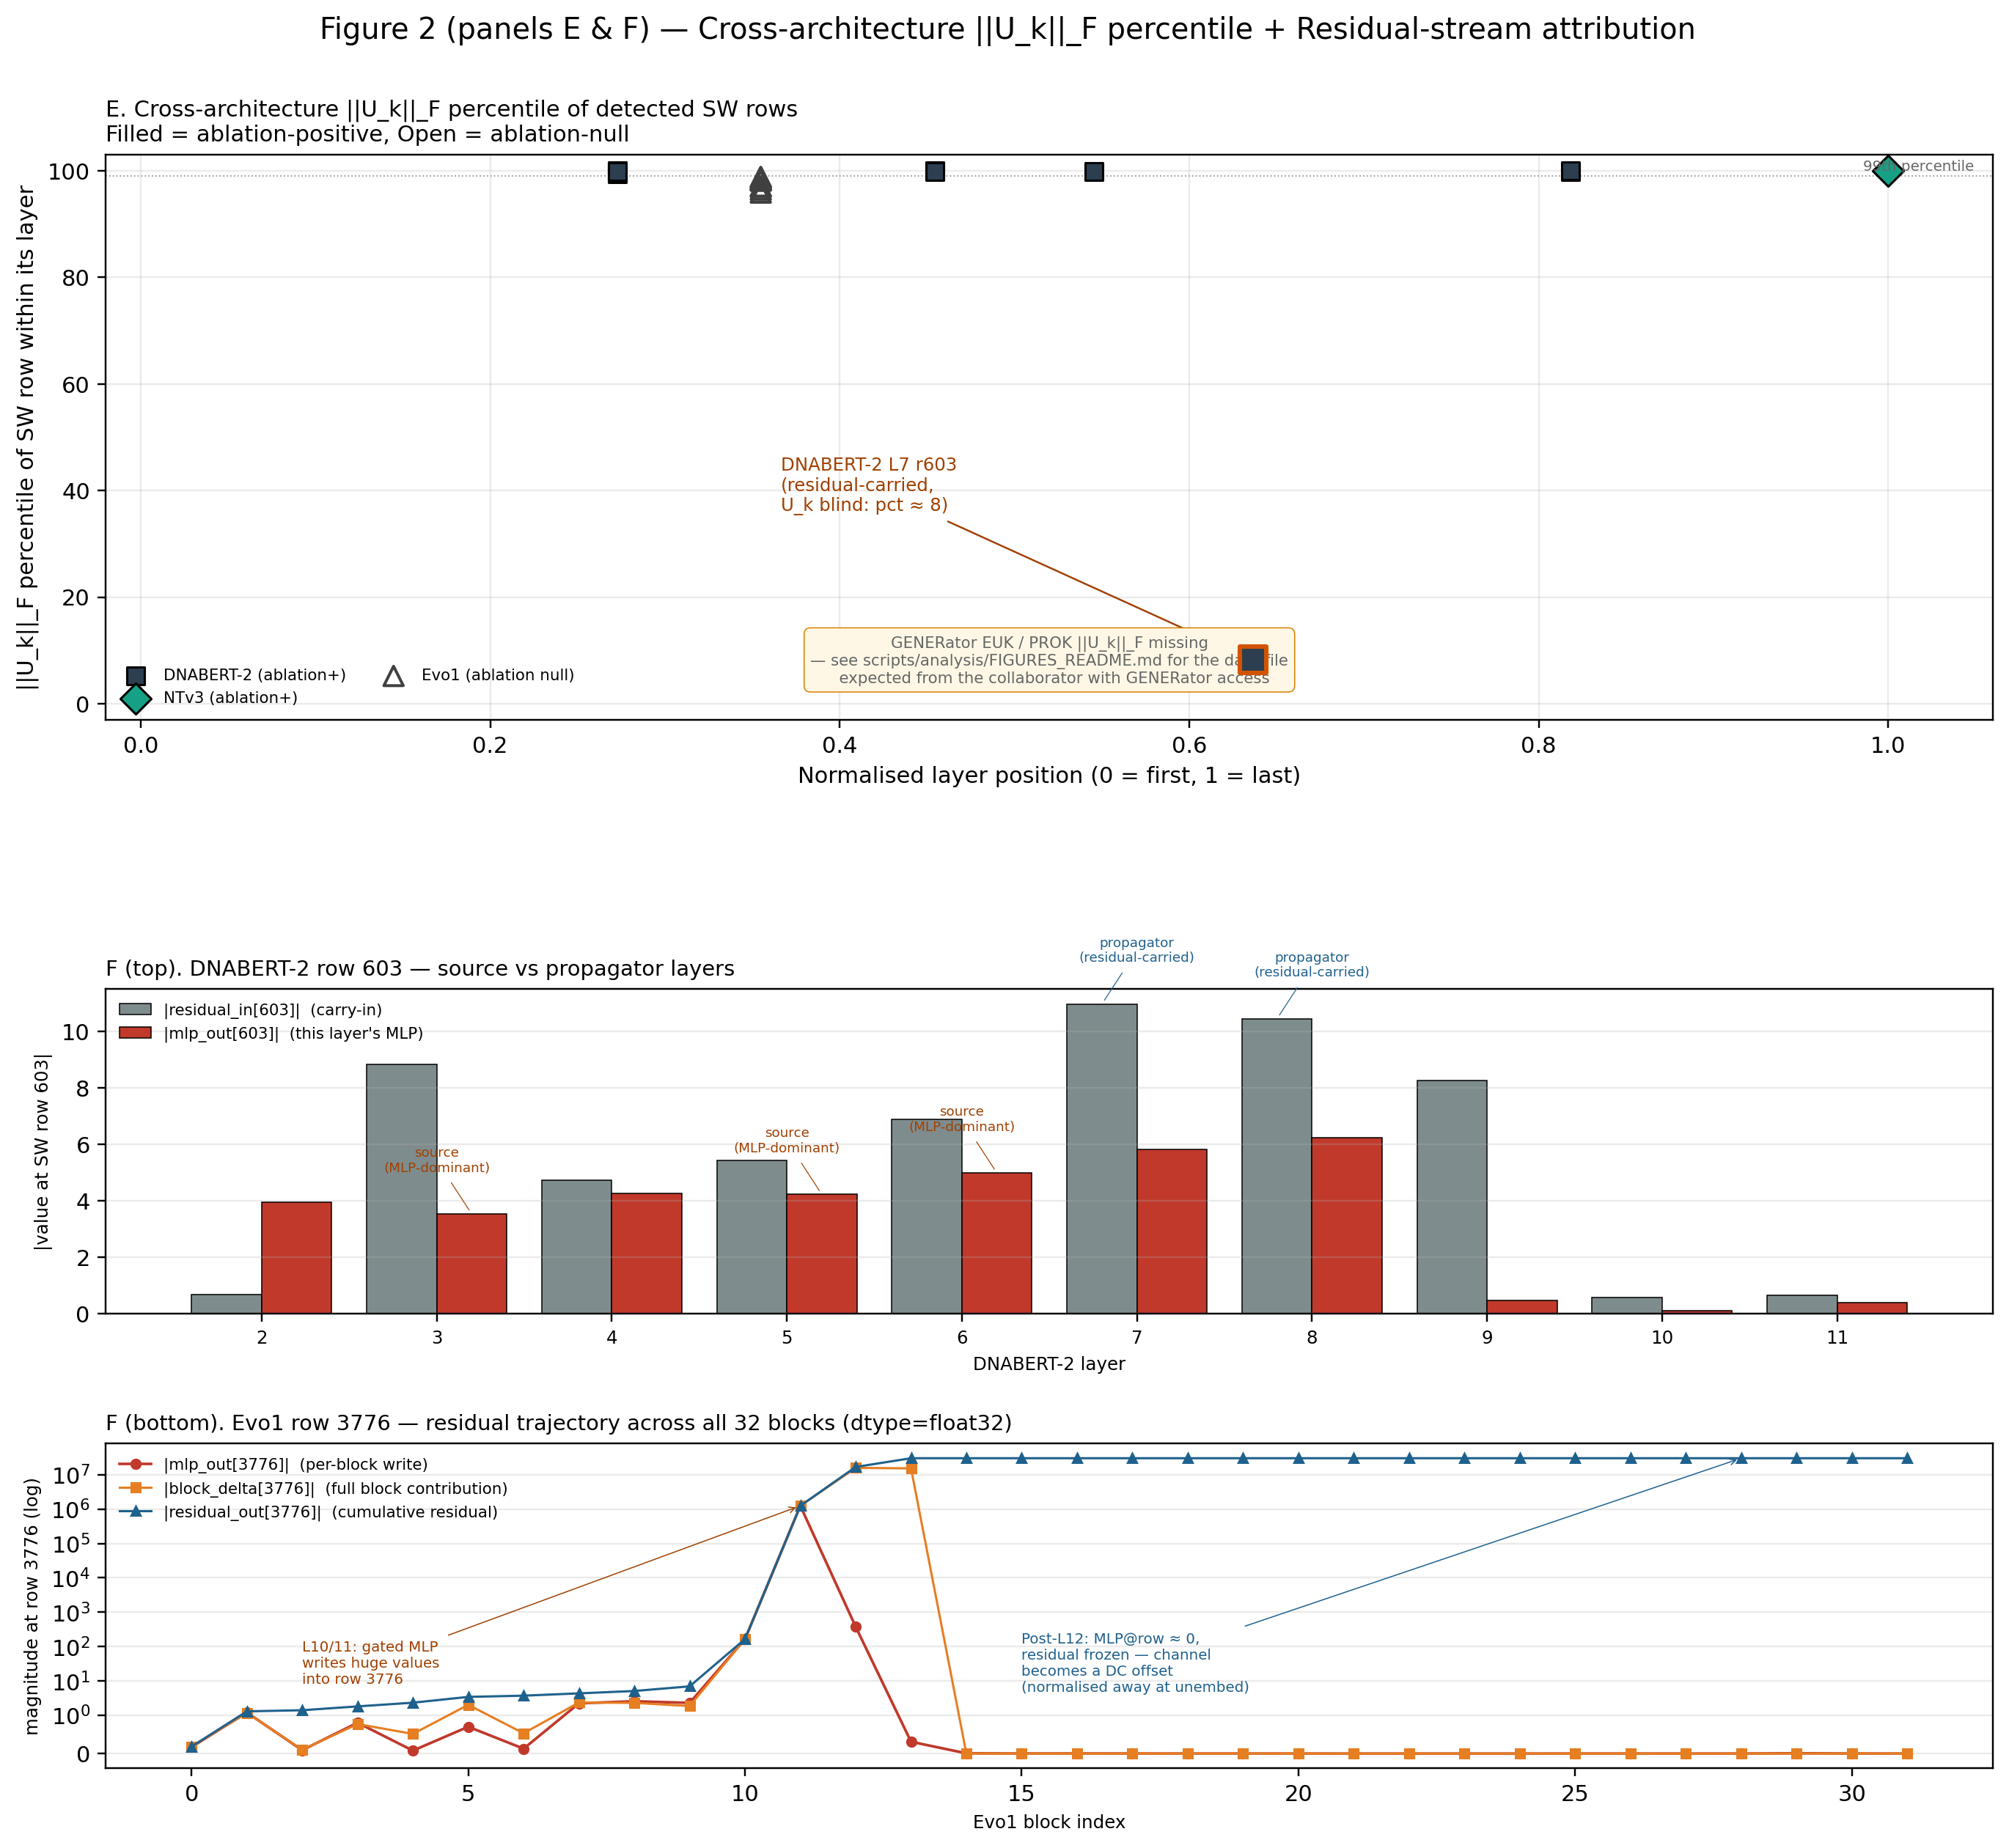
\includegraphics[width=\textwidth,height=0.62\textheight,keepaspectratio]{media/image_fig2_panels_EF.png}
\caption{\textbf{Cross-architecture $\|U_k\|_F$ predictor and
residual-stream attribution.}
(Panels A--D, GENERator EUK/PROK activation lifecycle and
step-up-layer $\|U_k\|_F$ bars, are pending GENERator JSONs and are
omitted from this render.)
\textbf{(E)}~$\|U_k\|_F$ percentile of the empirically identified SW
rows in DNABERT-2 (filled squares; 9 of 10 rows at the 99th+
percentile, 1 outlier at the 8th percentile), NTv3 (filled diamond;
rank 1/1{,}536 at L11), and Evo1 (open triangles; 95.9--98.8
percentile). GENERator markers drop in once the upstream JSONs land.
Filled markers indicate models where the SW row is load-bearing
under ablation; open markers indicate models where the same
predictor concentrates but ablation is null.
\textbf{(F)}~Residual-stream attribution at the SW token position.
Top: DNABERT-2 row 603 across layers 2--11, showing
$|\mathrm{mlp\_out}|$ and $|\mathrm{residual\_in}|$ per layer.
Layers 3, 5, 6 are MLP-dominant (source); layers 7--8 are
residual-dominant (propagator). At layer 9 the per-token argmax
shifts to row 264. Bottom: Evo1 row 3776 across all 32 StripedHyena
blocks (bf16-clean). At the source block, $|\mathrm{block\_delta}|
\approx |\mathrm{mlp\_out}|$ (ratio $\sim 1.0$); the residual is
faithfully deposited. Across subsequent blocks the row-aligned
magnitude attenuates while the global hidden-state magnitude is
preserved. The per-token argmax leaves row 3776 by layer~13.}
\label{fig:mech}
\end{figure}

\medskip
\noindent\textbf{Super-weights encode nucleotide composition with a
sign-reversed correlation across kingdoms}

Having established the structural mechanism and the dissociation
between architecture classes, we asked what each load-bearing SW
computes. We carried out the full causal-tracing, shuffle, hexamer,
motif-enrichment, regression, and sparse-autoencoder pipeline on
GENERator EUK and PROK, the two models where the concentrated
single-row phenotype permits clean perturbation. Across all
sequence-feature analyses, the SWs encoded nucleotide composition
rather than recognisable regulatory grammar, and the
SW-activation/ablation-cost correlation reversed sign between the
two kingdoms.

\textit{Causal necessity is context-uniform.}
We zeroed each model's SW row(s) during inference and measured loss
on 90 held-out sequences (30 each from promoters, enhancers, and
intergenic regions for EUK; promoters, terminators, and random for
PROK). In EUK, ablating rows 2{,}371 and 1{,}522 at layer~4
increased loss by $+2.92 \pm 1.33$ log-PPL units (promoter $+2.68$,
enhancer $+2.79$, random $+3.28$). In PROK, ablating row~1{,}927 at
layer~2 caused a larger increase of $+9.47$ log-PPL units (promoter
$+9.15$, terminator $+9.34$, random $+9.93$). Random control rows
produced shifts $< 0.0001$ log-PPL. Context-uniform degradation
across genomic classes is inconsistent with specialisation for a
single regulatory element class.

\textit{Shuffle controls separate the two kingdoms.}
We applied four shuffle controls (mononucleotide, dinucleotide,
trinucleotide, and 6-mer block) to each sequence and measured the
change in SW activation. In EUK, none of the four shuffles produced
a significant activation shift (all $p > 0.31$, $n = 90$); the
trinucleotide-preserving shuffle yielded $p = 0.841$. The EUK SW is
therefore consistent with token-identity-only encoding, with no
detectable sensitivity to sequence context above the individual
hexamer in this sample. In PROK, all four shuffles significantly
perturbed SW activation (mononucleotide $p = 0.0017$, dinucleotide
$p = 0.0092$, k-mer block $p = 0.0099$, trinucleotide $p < 10^{-8}$),
indicating context-sensitivity at multiple levels.

\textit{Sign-reversed SW-activation/ablation-cost correlation.}
A genome-wide scan over all 4{,}096 6-mers showed the EUK SW
activates broadly with a modest positive GC-content correlation
($r = +0.19$) and CC/CT-family k-mers at the top of the activation
distribution. We measured the KL divergence of the next-token
distribution before and after SW ablation for each hexamer. In EUK,
the Pearson correlation between SW activation and KL divergence was
$r = +0.437$ ($t = 5.06$, $p = 4.46 \times 10^{-7}$): hexamers that
strongly activate the SW are also those whose predictions are most
disrupted by its removal. AAAAAA, with activation~24, produced
near-zero KL on ablation (0.0018). In PROK the GC correlation is
negative ($r = -0.09$), AT-rich hexamers dominate the activation
distribution, and the SW-activation/KL-divergence correlation
reverses sign: $r = -0.710$ ($t = -118$, $p \approx 0$).
Top-quartile AT-rich activators in PROK produce a mean ablation KL
of 0.043, while bottom-quartile low-activation hexamers produce
KL $= 0.884$. We refer to the EUK pattern (high activation,
high ablation cost) as driver behaviour, and the PROK pattern (high
activation, low ablation cost) as suppressive-gate behaviour. Both
patterns are statistically robust within their respective model,
but we caution that the present data establish the correlation
reversal, not a fully resolved circuit-level account of why the two
kingdoms compute super-weights differently; a parallel EUK sparse
autoencoder (currently in training) is intended to give the same
basis-decomposition view of EUK that we have for PROK.

\textit{Sparse autoencoder decomposition of PROK independently
recovers the compositional axis.}
We trained a top-K sparse autoencoder ($k = 64$, dictionary size
12{,}288, $d_{\text{in}} = 3{,}072$) on residual-stream activations
from GENERator PROK at the step-up layer for 200{,}000 steps. The
SAE achieved high-fidelity reconstruction (MSE $= 4.78$ vs.\ random
baseline 7{,}238; 97.4\% of dictionary features active). Features
most positively correlated with SW magnitude ($r \approx {+}0.71$)
fired on GC-rich hexamers associated with coding and ribosomal
contexts (CGAGGT, ACCGAG, GACCAG, GGTCGG), while the most
anti-correlated features ($r \approx -0.73$ to $-0.76$) fired on
AT-rich and low-complexity sequences (AAAAAA, TTTTTG, GGGGGG). The
SAE thus recovers, from unsupervised sparse-dictionary learning on
residual-stream activations, the same GC/AT compositional axis that
the causal hexamer test identifies as predictive of ablation cost.
A subset of dictionary features were monosemantic but orthogonal to
the SW axis (\texttt{sw\_active\_frac} $= 0.0$), suggesting that the
SW's influence is encoded in distributed compositional features
rather than highly specific sequence detectors. The matched EUK SAE
encountered training instabilities and is the subject of follow-up
work.

\textit{No canonical regulatory motifs are enriched.}
We tested motif enrichment in the top-500 most SW-dependent k-mers
(ranked by KL divergence) against the remaining 3{,}596 using
Fisher's exact test with Benjamini--Hochberg correction. In EUK,
homopolymer-containing k-mers were the only significantly enriched
class (OR $= 1.85$, $q = 0.022$); splice donor, splice acceptor,
TATA-box, Kozak, CpG-rich, and GC-box motifs were all depleted or
at OR $\approx 1.00$ ($q = 1.00$). In PROK, no motif class survived
correction; Shine--Dalgarno, $-10$-box, and $-35$-box elements
showed no enrichment. SW dependency tracks a sequence-complexity
axis rather than recognisable biological regulatory grammar.

\textit{Sequence composition partially predicts ablation cost.}
OLS regression of $\Delta\mathrm{loss}$ on five composition features
(GC fraction, CpG density, k-mer entropy, repeat fraction,
complexity) explained $R^2 = 0.158$ in EUK and $R^2 = 0.347$ in
PROK. Sequence complexity ($\beta = -1.48$) and k-mer entropy
($\beta = +1.05$) dominate in EUK; GC fraction ($\beta = -0.306$)
and k-mer entropy ($\beta = -0.307$) in PROK. The modest variance
explained indicates that token-level identity, not high-level
summary statistics, drives most of the SW signal.

\textit{Super-weights are not kingdom-specific detectors.}
The EUK SW activated at 6{,}582 on hg38 and 6{,}610 on
\textit{E.~coli} (fold-change 1.004, Mann-Whitney $p = 0.538$); the
PROK SW at 10{,}638 on \textit{E.~coli} and 10{,}710 on hg38
($p = 0.644$). Neither row distinguishes between eukaryotic and
prokaryotic input.

\begin{figure}[H]
\centering

\includegraphics[width=\textwidth,keepaspectratio]{media/image_fig3.png}
\caption{\textbf{Super-weight encoding in GENERator EUK and PROK.}
\textbf{(A)}~Mean absolute SW activation grouped by hexamer
composition class (AT-rich, GC-rich, CpG-rich, homopolymer,
balanced) for EUK and PROK on a log axis.
\textbf{(B)}~EUK causal-hexamer scatter: SW activation ($x$) vs.\
KL divergence between clean and ablated next-token distributions
($y$) for all 4{,}096 hexamers; Pearson $r = +0.437$.
\textbf{(C)}~PROK causal-hexamer scatter, same axes; Pearson
$r = -0.710$.
\textbf{(D)}~Mean SW activation shift across four shuffle types
(mono-, dinuc-, trinuc-, 6-mer block) for EUK and PROK, with
per-shuffle $p$-values; EUK shifts are not statistically significant
at $n = 90$, PROK shifts are.
\textbf{(E)}~$\log_2$ odds ratio of motif-class enrichment in the
top-500 most SW-dependent hexamers vs.\ the remaining 3{,}596, for
EUK (right) and PROK (left). Only the EUK homopolymer-run class
reaches $q < 0.05$.}
\label{fig:kmer}
\end{figure}

\medskip
\noindent\textbf{Functional consequences in fine-tuned encoders}

DNABERT-2 shows only a $1.5\%$ perplexity increase on masked-LM
evaluation under SW-ensemble ablation; on this metric alone the
encoder would group with the SSM/hybrid negatives. To test whether
the SW ensemble matters for downstream applications, we fine-tuned
DNABERT-2 on three GUE benchmarks (promoter recognition,
splice-site detection, histone modification) and evaluated
SW-ablation effects across three random seeds.

Splice-site recognition dropped by $-25.5 \pm 0.7$ percentage points
($p = 0.0004$, one-sample $t$-test vs.\ zero), with random-row
controls $< 0.05$\,pp. Histone-modification prediction (H3K4me3)
was unaffected ($-4.5 \pm 6.2$\,pp, $p = 0.41$, n.s.). Promoter
recognition produced $-12.6 \pm 16.7$\,pp ($p = 0.40$, n.s.) with
strong seed dependence (seed~0: $-36.2\%$; seeds~1--2:
${\sim}{-}1\%$). The promoter result is therefore not statistically
distinguishable from zero at $n = 3$ seeds and we treat it as
inconclusive; it may reflect fine-tune-trajectory variance in
whether the model routes promoter-relevant computation through the
SW ensemble.

The same ablation protocol was applied to NTv3 on the splice task
across five random seeds (\textbf{Table~\ref{tab:ntv3}}). SW-row
ablation produced $\Delta\mathrm{MCC} = -0.119 \pm 0.054$
($t = -4.86$, $p = 0.008$ one-sample vs.\ zero; 5/5 seeds in the
negative direction); random-row controls produced
$|\Delta| < 3 \times 10^{-4}$. The damage magnitude varied across
seeds (range $-0.038$ to $-0.172$ in MCC). Seeds 0--2 showed
MCC degradation with corresponding accuracy drops; seeds 4--5
showed MCC collapse to near zero accompanied by an apparent
accuracy \emph{improvement} ($+0.05$, $+0.003$). Inspection of the
per-class confusion matrices showed that in seeds 4 and 5 the
SW-ablated model predicts the majority class on nearly every input,
raising accuracy toward the class-prior baseline
($\approx 0.55$--$0.57$) while eliminating discriminative ability
for the minority classes---exactly what MCC, which is invariant to
class prior, captures. We therefore report MCC as the primary
metric for NTv3 splice. We note that the choice of MCC was made
after observing seeds 4--5 and is therefore a post-hoc methodological
decision; we make it transparent here rather than retrofit the
narrative.

\begin{table}[H]
\centering\small
\begin{tabular}{cccccl}
\toprule
seed & base MCC & SW-abl MCC & $\Delta$MCC & $\Delta$Acc & class behaviour\\
\midrule
0 & 0.180 & 0.143 & $-0.038$ & $-0.057$ & mild damage\\
1 & 0.213 & 0.107 & $-0.106$ & $-0.247$ & strong damage\\
2 & 0.215 & 0.105 & $-0.111$ & $-0.124$ & strong damage\\
4 & 0.177 & 0.005 & $-0.172$ & $+0.050$ & collapse to majority class\\
5 & 0.184 & 0.018 & $-0.166$ & $+0.003$ & collapse to majority class\\
\midrule
mean & 0.194 & 0.075 & $-0.119$ & --- & 5/5 seeds negative $\Delta$MCC\\
s.d. & 0.019 & 0.061 & 0.054 & --- & $t = -4.86$, $p = 0.008$\\
\bottomrule
\end{tabular}
\caption{NTv3 splice-site SW ablation across five fine-tuning seeds.}
\label{tab:ntv3}
\end{table}

The splice/histone dissociation in DNABERT-2 is consistent with the
SW's role as a local-hexamer detector: splice donor and acceptor
sites are defined by short consensus sequences with CC/CT-rich
flanking context, while H3K4me3 reflects chromatin state correlated
with diffuse genomic context rather than local hexamer identity.
This is a post-hoc reading of the result rather than an independent
test, but it is consistent with the EUK SW's k-mer scan.

To distinguish bottleneck from ensemble behaviour we ablated each of
the ten DNABERT-2 SW rows individually on the fine-tuned splice
checkpoint. The maximum single-row effect was $-1.45\%$ accuracy
(row L3 r603); the activation-detected top row (L5 r603,
out\_max $= 944.6$) caused only $-0.15\%$. Removing all ten together
produces the full $-25.5\%$ collapse. The DNABERT-2 super-weights
therefore act as a functionally redundant ensemble, in contrast to
GENERator's single dominant row that alone produces $+23{,}000\%$
PPL loss. The ten encoder SW rows share only six unique row indices
across five layers, with row 603 alone recurring at layers 3, 5, 6,
and 7, consistent with the residual-stream channel reuse documented
in the mechanism section.

\begin{figure}[H]
\centering

\includegraphics[width=\textwidth,keepaspectratio]{media/image_fig4.png}
\caption{\textbf{Functional consequences of SW ablation in fine-tuned
encoders.}
\textbf{(A)}~DNABERT-2 GUE task performance after SW-ensemble
ablation vs.\ random-row control, mean $\pm$ s.d.\ across 3 seeds.
\textbf{(B)}~NTv3 splice-site ablation across 5 seeds. Per-seed base
MCC and SW-ablated MCC are shown side by side; seeds 4 and 5 show
near-zero post-ablation MCC despite positive $\Delta$Acc due to
majority-class collapse (see Table~\ref{tab:ntv3}).
\textbf{(C)}~Per-row ablation on the DNABERT-2 splice checkpoint:
the maximum single-row effect is $-1.45\%$ accuracy; the full effect
requires removing all ten rows together.}
\label{fig:gue}
\end{figure}

\medskip
\noindent\textbf{Implications for model compression}

The SW structure has implications for which parameters in a
transformer genomic LM are safely compressible. The Yu et al.\
heuristic for NLP\textsuperscript{10} prescribes retaining SW rows
in full precision and quantizing everything else uniformly. In
contrast, we find that SW proximity stratifies rows by compression
sensitivity in a more graded manner: rows distant from any SW
coordinate are uniquely fragile under pruning, while the $\|U_k\|_F$
structural predictor provides a weight-only criterion for precision
allocation under quantization.

\textit{Far-from-SW rows are uniquely fragile under pruning.}
We performed a progressive row-pruning sweep on DNABERT-2 fine-tuned
on core-promoter recognition (baseline accuracy 83.46\%, MCC
0.670), zeroing increasing fractions of \texttt{down\_proj} rows
(0.5\%--30\%) selected by five criteria: L1-low, L1-high, prox-near
(closest in (layer, row) space to the SW coordinates), prox-far
(most distant), and random (mean of 10 seeds). At 20\% of rows
pruned, prox-near lost $-1.60$\,pp, while prox-far lost
$-9.39$\,pp---a 5.9-fold difference (Fig.~\ref{fig:compression}A).
At 30\% the asymmetry persists ($-1.65$ vs.\ $-8.15$\,pp). Random
pruning at matched count produced only $-0.82$\,pp at 20\% and
$-1.38$\,pp at 30\%, indicating that near-SW rows are slightly
\emph{more} important than average rather than shadow-redundant.
The dominant signal is therefore far-SW fragility, not near-SW
tolerance: rows most distant from the SW coordinate are those the
model relies on most for tasks unrelated to the SW's compositional
function. Magnitude-based criteria (L1-low $-3.93$\,pp, L1-high
$-1.20$\,pp at 30\%) fall between random and far-SW extremes.

\textit{Quantization sensitivity in GENERator.}
We applied per-row round-to-nearest (RTN) INT4 quantization to
GENERator's MLP \texttt{down\_proj} matrices across five conditions
on a held-out hg38 perplexity benchmark. INT4 quantization of all
92{,}158 non-SW rows costs $+0.159$ PPL nats. Quantizing the two SW
rows alone is essentially free ($-0.013$ PPL, n.s.). At 30\%
near-SW quantization (27{,}647 rows), PPL decreases by $-0.023$
nats, while random-row quantization at matched count produces
$+0.044 \pm 0.037$ ($t = -5.68$, $p = 0.0003$ across 10 seeds). The
near-SW effect is robust across fractions 10--30\% ($p \leq 0.016$
at every fraction) and absent at INT8. Near-SW rows tolerate INT4
better than random rows in this perplexity-level evaluation.

\textit{U$_k$-guided precision allocation on downstream tasks.}
We extended the INT4 evaluation to DNABERT-2 on three GUE
downstream tasks---splice (SW-dependent), promoter core (moderate),
and histone H3K4me3 (SW-independent)---across three quantization
fractions (10, 20, 30\%) with five seeds per stochastic condition.
We compared six selection strategies: near-SW, far-SW, random,
$\|U_k\|_F$-low, $\|U_k\|_F$-high, and the Yu heuristic (all
non-SW rows). At fractions $\leq 30\%$, all conditions caused
$\leq 0.003$ accuracy degradation on every task, confirming that
INT4 quantization of any row subset at these fractions is safe
on DNABERT-2 regardless of criterion. However, on the two tasks
where SW ablation has weak or no functional effect (promoter core,
histone), quantizing rows with low $\|U_k\|_F$ consistently
outperformed quantizing rows with high $\|U_k\|_F$; the advantage
reached $+0.0038$ accuracy at 20\% on histone
(Fig.~\ref{fig:compression}B). On splice, where the SW ensemble
is directly load-bearing, the $\|U_k\|_F$ guidance was confounded
by SW rows with anomalously low $\|U_k\|_F$ (e.g.\ layer~7
row~603 at the 8th percentile) and showed no consistent advantage.
The same structural criterion---$\|U_k\|_F$ computed from cold
weights without any forward pass---that identifies candidate
super-rows also predicts INT4 sensitivity on SW-independent tasks,
providing a principled, weight-only criterion for precision
allocation at deployment time.

\textit{Whole-model INT4 with SW exemption.}
We extended the test to full model scope (all seven projection
types; 806{,}396--806{,}400 rows across 30 layers) on a
$\sim 100{,}000$-token hg38 probe. INT4 quantization of all non-SW
eligible rows produced $+0.0879$ PPL on EUK (baseline 8.427) and
$+0.4664$ PPL on PROK (baseline 8.783). Including the SW rows in
the quantization pool changed the result by $-0.0008$ PPL on EUK
and $+0.0004$ PPL on PROK; SW-only fragility was correspondingly
small ($+0.00013$ PPL on EUK, $-0.00007$ PPL on PROK). At this
evaluation power, the SW marginal cost is below the noise floor of
the broader INT4 cost. We interpret this as evidence that protecting
the SW row alone confers no measurable benefit in these models, in
contrast to the Yu et al.\ NLP finding; we do not interpret it as
ruling out a benefit at finer perplexity resolution.

\begin{figure}[H]
\centering

\includegraphics[width=\textwidth,keepaspectratio]{media/image_fig5.png}
\caption{\textbf{Compression behaviour around the super-weight
neighbourhood.}
\textbf{(A)}~Progressive \texttt{down\_proj} row-pruning sweep on
DNABERT-2 (5 selection criteria, 0.5--30\% of non-SW rows).
Far-from-SW rows are uniquely fragile (5.9\,$\times$ worse than
near-SW at 20\%); random-row pruning produces less degradation than
near-SW pruning.
\textbf{(B)}~U$_k$-guided INT4 across three GUE tasks at 20\%
fraction. Rows with low $\|U_k\|_F$ tolerate INT4 better than rows
with high $\|U_k\|_F$ on SW-independent tasks (promoter-core,
histone); on splice (SW-dependent) the effect is absent due to
SW-outlier confounding.
\textbf{(C)}~Whole-model INT4 with and without SW exemption on a
$\sim 100{,}000$-token hg38 probe; the SW marginal cost is
indistinguishable from zero.}
\label{fig:compression}
\end{figure}

\textbf{Discussion}

Super-weights in the genomic language models we tested are not a
universal property of large-scale sequence modelling; they are
present in transformer-class architectures with gated FFNs and
attention-style mixing, and absent in StripedHyena under the same
detect-then-ablate protocol. The main mechanistic contribution of
this work is the identification of $\|U_k\|_F$ as a structural
predictor of candidate super-rows that holds across two encoder
topologies and one decoder topology, from cold weights and without
any forward pass. The same predictor concentrates on candidate rows
in Evo1 but those candidates are not load-bearing, which we
interpret as a separable systemic property of the surrounding mixer.
We are explicit that this decomposition is currently supported by
one positive$\to$negative architecture transition (gated-FFN
transformer to StripedHyena) and is therefore a working hypothesis;
extending it to other non-attention mixers (Mamba, EMA, parallel
Hyena variants) is the natural next test.

Within the SW-positive models, the super-weight encodes nucleotide
composition rather than annotated regulatory grammar. The
SW-activation/ablation-cost correlation reverses sign between
GENERator EUK and PROK ($r = +0.437$ vs.\ $r = -0.710$), and a
sparse autoencoder trained on PROK residual-stream activations
recovers the same GC-rich vs.\ AT-rich axis. We refer to these as
driver vs.\ suppressive-gate behaviours and are explicit that what
we have characterised is the correlation reversal, not a fully
resolved circuit-level account; a matched EUK SAE is in progress.

Functionally, the DNABERT-2 SW ensemble is required for splice-site
recognition ($-25.5\%$ accuracy across 3 seeds) but not for
histone-mark prediction; the splice effect replicates in NTv3 across
five seeds (5/5 negative direction, $p = 0.008$ on MCC). The
splice/histone dissociation is consistent with a local-hexamer
detector role for the SW ensemble (splice sites have short
consensus sequences; H3K4me3 reflects diffuse chromatin context)
and provides a usable diagnostic principle: tasks that depend on
short consensus motifs are likely to route through the SW ensemble,
and tasks that depend on diffuse signal are less likely to.

The compression results reveal a graded picture of SW-proximity
effects that differs from the Yu et al.\ heuristic in two respects.
First, pruning tolerance is stratified by SW distance, with
far-from-SW rows being uniquely fragile (5.9\,$\times$ worse than
near-SW at 20\%) while random pruning is safer than near-SW pruning.
The dominant signal is far-SW fragility, not near-SW tolerance.
Second, INT4 quantization of any row subset at fractions
$\leq 30\%$ caused negligible accuracy degradation on all three
downstream tasks tested, and the $\|U_k\|_F$ structural predictor
provided a principled, weight-only precision-allocation criterion
that outperformed random selection on SW-independent tasks. A
hardware-INT4 throughput evaluation on multiple downstream tasks
is the natural follow-up.

\textit{Limitations.}
We note several limitations explicitly. First, the
structural-vs-systemic decomposition rests on a single architecture
transition (gated-FFN transformer to StripedHyena hybrid via Evo1);
direct replication on Evo2, MegaDNA, HybridNA, and on Mamba-class
models is a revision-stage goal. Second, the kingdom-asymmetric
sign reversal is established between two GENERator models trained
on different corpora with otherwise matched architecture and
training procedure, but we have not run the same comparison on
other transformer-decoder genomic LMs to confirm that the reversal
generalises beyond GENERator. Third, the disentanglement of
architecture from tokenizer is incomplete: GENERator uses 6-mer
tokenization and is SW-positive, Evo1/Evo2 use byte-level
tokenization and are SW-negative under ablation; a publicly
available byte-level transformer decoder for genomics would
disambiguate this. Fourth, the GENERator EUK SAE encountered
training instabilities and is incomplete; only the PROK SAE result
is currently in this manuscript. Fifth, the DNABERT-2 promoter
result is seed-dependent and not statistically distinguishable from
zero at $n = 3$; we report it as inconclusive rather than positive.
Sixth, the MCC-over-accuracy choice for NTv3 splice was made after
observing seeds 4 and 5 collapse to majority class; we report this
metric decision transparently rather than retrofit the narrative.

\textbf{Methods}

\textit{Models.}
GENERator eukaryote 3B
(\texttt{GenerTeam/GENERator-v2-eukaryote-3b-base}) and GENERator
prokaryote 3B (\texttt{GenerTeam/GENERator-v2-prokaryote-3b-base})
are Llama-style causal decoders (30 layers, $d_{\text{model}} =
3{,}072$, $d_{\text{ffn}} = 8{,}448$, vocabulary 4{,}128, 6-mer BPE
tokenisation). DNABERT-2 117M (\texttt{zhihan1996/DNABERT-2-117M})
is a BERT-style encoder (12 layers, $d_{\text{model}} = 768$,
$d_{\text{ffn}} = 3{,}072$, vocabulary 4{,}096, BPE). NTv3 50M,
Evo1 7B, Evo2 7B (loading-blocked), MegaDNA, HybridNA, and
Caduceus-PS were loaded from HuggingFace Hub in full precision
where compatible.

\textit{Detect-then-ablate protocol.}
Forward hooks recorded $\max|\mathrm{input}|$ and
$\max|\mathrm{output}|$ per layer at the down-projection (or
architectural analogue: \texttt{model.layers.\{i\}.mlp.down\_proj}
for GENERator; \texttt{model.encoder.layer.\{i\}.intermediate.dense}
for DNABERT-2; \texttt{l3} of \texttt{ParallelGatedConvBlock} for
Evo1) over a 48-bp probe sequence. The layer with the globally
largest $\max|\mathrm{input}|$ is the spike layer; its out-channel
is the candidate SW row. We iteratively zeroed $W[r,c]$ and re-ran
the sweep until $\max|\mathrm{input}| < 10\%$ of the initial value
or 10 iterations. The detection criteria are identical across
models; the functional readout differs by model type (held-out
perplexity for causal LMs; held-out perplexity plus fine-tuned GUE
accuracy/MCC for masked encoders that admit downstream tasks).

\textit{Quadratic amplifier audit.}
For each output coordinate $k$ of any gated FFN:
\[
\|U_k\|_F
= \sqrt{\sum_{i=1}^{d_{\text{ffn}}}
  W_{\text{down}}[k,i]^2
  \cdot \|W_{\text{gate}}[i,:]\|^2
  \cdot \|W_{\text{up}}[i,:]\|^2}.
\]
The formula applies to SwiGLU
($W_{\text{gate}}, W_{\text{up}}, W_{\text{down}}$ as named in
GENERator), to DNABERT-2's \texttt{BertGatedLinearUnitMLP} (gate and
up packed on adjacent row blocks of \texttt{gated\_layers}; down
projection is \texttt{wo}), to NTv3's gated FFN, and to Evo1's
\texttt{ParallelGatedConvBlock} (\texttt{l1}/\texttt{l2}/\texttt{l3}
as gate/up/down). All audits are performed from cold model weights
with no forward pass.

\textit{Residual-stream attribution.}
At the SW token position we recorded the pre-block residual
$H_i[:, \mathrm{SW\_row}]$ and the MLP contribution
$\Delta_i^{\mathrm{MLP}}[:, \mathrm{SW\_row}]$ at each layer using
forward pre-hooks and post-hooks. A layer is classified as a source
if $|\Delta_i^{\mathrm{MLP}}| > |H_i|$ at the SW row and as a
propagator otherwise. The Evo1 trace was run in bf16 across all 32
StripedHyena blocks.

\textit{Causal ablation.}
A PyTorch forward hook zeros the SW row(s) at the
\texttt{down\_proj} output on every forward pass. We report mean
per-token cross-entropy loss (nats) from the HuggingFace CausalLM
forward pass with \texttt{labels=input\_ids} on 30 non-overlapping
3{,}072-bp windows from \textit{E.~coli} K-12 (PROK) or hg38 (EUK).

\textit{Shuffle controls.}
Four variants: mononucleotide; dinucleotide-preserving
(Altschul--Erickson De Bruijn); trinucleotide-preserving;
6-mer block (shuffle at the hexamer-token level).

\textit{Hexamer scan and causal hexamer test.}
For each 6-mer token, an 11-token context (5 flanking poly-A) is
passed through the model; the SW row activation is recorded.
$D_{\mathrm{KL}}(p\|q) = \sum_v p_v \log(p_v/q_v)$ with
$\varepsilon = 10^{-9}$ added before renormalisation.

\textit{Motif enrichment.}
Top-500 hexamers by KL divergence tested against the remaining
3{,}596 by two-sided Fisher exact test with Benjamini--Hochberg
correction. Eukaryotic and prokaryotic motif classes as previously
described.

\textit{Activation lifecycle.}
Pre-hooks and post-hooks on every transformer layer capture the
post-residual hidden state $H_{i+1}$; we extract
$\max_t |H_i[:,k]|$ for SW row $k$ at layer $i$, averaged over 20
sequences of 504~nt.

\textit{DNABERT-2 and NTv3 GUE fine-tuning and ablation.}
DNABERT-2 fine-tuning on three GUE tasks
(\texttt{prom/prom\_core\_notata}, \texttt{splice/reconstructed},
\texttt{EMP/H3K4me3}) with three random seeds (0, 1, 2). NTv3
fine-tuning on \texttt{splice/reconstructed} with five random seeds
(0, 1, 2, 4, 5; seed 3 was excluded due to a non-converging
training run). SW-row ablation applied at evaluation time via
forward hooks on the fine-tuned checkpoint; matched random-row
controls use 10 random row sets per seed. We report MCC as the
primary metric for NTv3 splice because seeds 4 and 5 showed
majority-class collapse under SW ablation; this metric choice was
made after observing the seed behaviour and is reported here rather
than retrofit into the main narrative.

\textit{Pruning sweep.}
Five ranking criteria (L1-low, L1-high, prox-far, prox-near,
random) over fractions $\{0.5, 1, 2, 5, 10, 15, 20, 30\}\%$ of the
non-SW \texttt{down\_proj} row pool. Random reports mean $\pm$ std
over 10 seeds.

\textit{INT4 quantization.}
Per-row RTN with symmetric scale:
$\hat{r} = \mathrm{round}(r/s)\cdot s$, $s = \max|r|/7$, integer
range $[-7,7]$. The whole-model variant quantises all seven
projection types across 30 layers (806{,}396--806{,}400 rows) on
$\approx 100{,}000$ tokens. SW marginal cost is
$\Delta_{\mathrm{Yu+SW}} - \Delta_{\mathrm{Yu\text{-}exempt}}$.

\textit{Sparse autoencoder.}
Top-K sparse autoencoder ($k = 64$, dictionary size 12{,}288, input
dimension 3{,}072) trained on residual-stream activations from
GENERator PROK at layer 2 for 200{,}000 steps. Feature--SW
correlation is computed as Pearson $r$ between per-hexamer feature
activation and SW magnitude across all 4{,}096 6-mers.

\textbf{References}

\begin{enumerate}[leftmargin=*,label={[\arabic*]}]

\item Avsec, \v{Z}.\ et al. Effective gene expression prediction
from sequence by integrating long-range interactions.
\textit{Nat.\ Methods} \textbf{18}, 1196--1203 (2021).

\item Dalla-Torre, H.\ et al. Nucleotide Transformer: building and
evaluating robust foundation models for human genomics.
\textit{Nat.\ Methods} \textbf{22}, 287--297 (2025).

\item Linder, J., Srivastava, D., Yuan, H., Agarwal, V.\ \&
Kelley, D.\,R. Predicting RNA-seq coverage from DNA sequence as a
unifying model of gene regulation. \textit{Nat.\ Genet.}
\textbf{57}, 949--961 (2025).

\item Wu, W.\ et al. GENERator: A Long-Context Generative Genomic
Foundation Model. Preprint (2025).

\item Boshar, S.\ et al. A foundational model for joint
sequence-function multi-species modeling at scale for long-range
genomic prediction. \textit{bioRxiv} 2025.12.22.695963 (2025).

\item Zhou, Z.\ et al. DNABERT-2: Efficient Foundation Model and
Benchmark For Multi-Species Genome. Preprint (2023).

\item Brixi, G.\ et al. Genome modelling and design across all
domains of life with Evo~2. \textit{Nature} \textbf{652},
1349--1361 (2026).

\item Ma, M.\ et al. HybriDNA: A Hybrid Transformer-Mamba2
Long-Range DNA Language Model. Preprint (2025).

\item Shao, B.\ \& Yan, J. A long-context language model for
deciphering and generating bacteriophage genomes.
\textit{Nat.\ Commun.} \textbf{15}, 9392 (2024).

\item Yu, M., Wang, D., Shan, Q., Reed, C.\,J.\ \& Wan, A. The
Super Weight in Large Language Models. Preprint arXiv:2411.07191
(2024).

\item Sun, P.\ et al. The Spike, the Sparse and the Sink: Anatomy
of Massive Activations and Attention Sinks. Preprint
arXiv:2603.05498 (2026).

\end{enumerate}

\end{document}